\documentclass[11pt,a4paper]{article}
\usepackage[utf8]{inputenc}
\usepackage{amsmath,amssymb,amsfonts,amsthm}
\usepackage{geometry}
\usepackage{graphicx}
\usepackage{hyperref}
\usepackage{listings}
\usepackage{xcolor}
\usepackage{booktabs}
\usepackage{microtype}
\usepackage{tabularx}
\usepackage{enumitem}
\usepackage{caption}
\usepackage{subcaption}
\usepackage{colortbl}

\geometry{margin=1in}

% --- Color Palette ---
\definecolor{primaryblue}{RGB}{24, 76, 120}
\definecolor{darknavy}{RGB}{10, 30, 60}
\definecolor{codegreen}{rgb}{0,0.6,0}
\definecolor{codegray}{rgb}{0.5,0.5,0.5}
\definecolor{codepurple}{rgb}{0.58,0,0.82}
\definecolor{backcolour}{rgb}{0.96,0.96,0.96}
\definecolor{bordergray}{rgb}{0.85,0.85,0.85}
\definecolor{excalibg}{RGB}{245, 247, 250}

\hypersetup{
    colorlinks=true,
    linkcolor=primaryblue,
    citecolor=primaryblue,
    urlcolor=primaryblue
}

\lstdefinestyle{mystyle}{
    backgroundcolor=\color{backcolour},   
    commentstyle=\color{codegreen},
    keywordstyle=\color{primaryblue}\bfseries,
    numberstyle=\tiny\color{codegray},
    stringstyle=\color{codepurple},
    basicstyle=\ttfamily\footnotesize,
    breakatwhitespace=false,         
    breaklines=true,                 
    captionpos=b,                    
    keepspaces=true,                 
    numbers=left,                    
    numbersep=6pt,                  
    showspaces=false,                
    showstringspaces=false,
    showtabs=false,                  
    tabsize=2,
    frame=single,
    rulecolor=\color{bordergray}
}
\lstset{style=mystyle}

\newenvironment{excalidrawbox}{%
  \begin{center}%
  \begin{tabular}{|p{0.93\textwidth}|}
  \hline
  \rowcolor{excalibg}%
}{%
  \\ \hline
  \end{tabular}%
  \end{center}%
}

\title{\Huge \textbf{KernelLens: Deploying Triton Kernels to C++ Inference Engines} \\[0.5em]
\large \textit{Automated ONNX Runtime \& TensorRT Plugin Synthesis for Production Deep Learning Operators}}

\author{
    \textbf{Justin Duc} \\
    \textit{Galiad Research}
}
\date{\today}

\begin{document}

\maketitle

\begin{abstract}
Writing custom high-performance GPU kernels using OpenAI Triton has become the dominant paradigm for authoring state-of-the-art deep learning operators. However, deploying models containing custom Python \texttt{@triton.jit} kernels into production enterprise C++ inference runtimes---specifically Microsoft ONNX Runtime (ORT) and NVIDIA TensorRT (TRT) 10.x---presents severe architectural barriers. Standard ONNX graph export mechanisms cannot trace imperative Python Triton calls, dynamic launch grid functions, implicit layout semantics, in-place memory mutability, dynamic runtime host scalars, or low-level PTX entry parameter signatures.

In this paper, we present \textbf{KernelLens v1.1.9}, an end-to-end automated compilation, C++/CUDA code synthesis, and zero-copy runtime framework. KernelLens bridges arbitrary PyTorch models containing custom Triton kernels directly to high-throughput ONNX Runtime and TensorRT custom C++ plugins with zero manual C++ development. We present an exhaustive 12-step technical formalization of KernelLens's core compiler pipeline: (1)~User Model \& Kernel Signature Inspection; (2)~Target Engine Configuration; (3)~Pass 1 Concrete Eager GPU Execution \& PTX Artifact Interception; (4)~Pass 2 Symbolic FX Proxy Tracing \& SymPy Grid Expression Extraction; (5)~Static AST Inspection of Main \& Recursive Nested Helper Functions; (6)~Manifest Validation; (7)~Base ONNX Export \& Domain Custom Node Injection (\texttt{triton\_custom::<name>}); (8)~Host-Side Dynamic Scalar Binding (\texttt{OrtMemTypeCPUInput}); (9)~Automated C++/CUDA Code Generation (\texttt{ort\_gen.py}, \texttt{trt\_gen.py}); (10)~16-Byte Hardware Memory Alignment Guard Insertion ($\text{Address} \pmod{16} == 0$); (11)~Native \texttt{nvcc}/\texttt{g++} Shared Library Compilation (\texttt{.so}); and (12)~Dynamic Plugin Registration with Zero-Copy VRAM IO Binding.

We detail key architectural innovations in v1.1.9, including: (a)~TensorRT 10.16 C++ plugin dynamic creators with explicit symbol registration (\texttt{register\_triton\_plugins\_explicit}) enforcing \texttt{kLINEAR} tensor formats; (b)~Automated Blackwell (\texttt{sm\_120a}) PTX 9.0 ISA version clamping (\texttt{.version 9.3} $\rightarrow$ \texttt{.version 9.0}) to satisfy CUDA 13.0 driver JIT requirements; (c)~Primary CUDA context retention (\texttt{cuDevicePrimaryCtxRetain}) to prevent multi-threaded context detachment; and (d)~Executable stack security clearance (\texttt{patchelf}) for Linux 7.0 kernels. We evaluate KernelLens across state-of-the-art research model kernels from \textbf{LLaMA 3}, \textbf{Mistral}, \textbf{Qwen 2.5}, \textbf{PaLM}, and \textbf{Liger-Kernel} (Fused RMSNorm, SwiGLU, Rotary Position Embeddings, and Fused Cross-Entropy Loss). KernelLens achieves \textbf{exact floating-point numerical parity} ($\text{MaxDiff} = 0.00\text{e}+00$) against eager Triton execution while enabling production-grade C++ inference deployment.
\end{abstract}

\tableofcontents
\newpage

% =========================================================================
\section{Introduction}
% =========================================================================

Deep learning systems increasingly rely on domain-specific GPU kernels to achieve peak computational efficiency, reduce VRAM bandwidth demands, and fuse multi-stage attention and normalization blocks. OpenAI Triton \cite{triton2019} has established itself as the standard programming model for authoring custom GPU kernels in Python, providing C/CUDA-like execution control with Python syntax.

Despite Triton's widespread adoption in model authoring and training, a major infrastructure friction point emerges when transitioning models to production deployment. Enterprise deployment pipelines standardly deploy models within specialized C++ execution engines, such as \textbf{Microsoft ONNX Runtime (ORT)} \cite{onnxruntime} and \textbf{NVIDIA TensorRT (TRT)} \cite{tensorrt}, to achieve low latency, stream concurrency, and hardware-specific kernel graph optimizations.

Deploying PyTorch models containing custom \texttt{@triton.jit} kernels directly into ONNX Runtime or TensorRT fails due to six critical architectural gaps:
\begin{enumerate}
    \item \textbf{ONNX Exporter Tracing Breakdown:} Standard PyTorch ONNX export utilities (\texttt{torch.onnx.export}) operate on TorchScript or TorchDynamo IRs representing native PyTorch C++ operators (\texttt{at::native}). Imperative Python calls to \texttt{triton.JITFunction} instances are opaque to PyTorch's trace backend, leading to immediate tracing failure or missing graph nodes.
    \item \textbf{Dynamic Launch Grid Resolution:} Triton launch grids are defined via dynamic Python lambda functions $\text{grid}(x, y, z) = (g_x(s_i), g_y(s_i), g_z(s_i))$ dependent on runtime tensor dimensions $s_0, s_1, \dots$. Standard graph representations cannot symbolize or execute arbitrary Python grid lambdas inside standalone C++ engines.
    \item \textbf{PTX Entry Signature Mismatch:} The Triton LLVM backend compiles Python source code directly into Parallel Thread Execution (PTX) assembly code. The resulting PTX entry declarations (\texttt{.entry <kernel> (.param .u64 p0, ...)}) re-order parameters, drop unused arguments, and enforce specific bitwidths. Native C++ plugin wrappers must dynamically align host argument pointers to match PTX signatures exactly.
    \item \textbf{Nested Code \& In-Place Mutability Analysis:} Research kernels frequently delegate memory store and load operations to nested Python helper functions or perform in-place buffer mutations ($\text{ptr}_{\text{out}} \equiv \text{ptr}_{\text{in}}$). Static compilers fail to track nested mutation semantics, producing corrupted outputs or invalid graph topologies.
    \item \textbf{Dynamic Runtime Host Scalar Arguments:} Practical models pass scalar arguments (e.g., scaling factors $\alpha$, soft-cap limits $\tau$) that change per forward pass. C++ execution engines must accept host-side CPU scalar arguments without triggering costly kernel recompilation.
    \item \textbf{16-Byte Hardware Memory Alignment Bounds:} Vectorized GPU memory instructions (\texttt{ld.global.v4.b32}) strictly require starting VRAM pointers to satisfy 16-byte alignment ($\text{Address} \pmod{16} == 0$). Standard inference allocators may provide sub-aligned memory buffers, causing hardware misaligned address exceptions (\texttt{CUDA error 716}).
\end{enumerate}

To bridge this gap, we present \textbf{KernelLens}, a comprehensive compilation and runtime synthesis system. KernelLens allows machine learning engineers to write custom PyTorch Triton kernels in pure Python, compile the entire model into optimized ONNX computational graphs paired with C++ custom operator shared libraries (\texttt{.so}), and execute them inside ONNX Runtime and TensorRT with zero manual C++ programming.

\subsection{The Core Value Proposition: Full Graph Optimizations with Custom Triton Kernels}

In enterprise deep learning production, real-world models (e.g., LLaMA 3, Mistral, Qwen 2.5, Flux, DeepSeek) are structural hybrids. They consist of:
\begin{enumerate}[leftmargin=1.5em]
    \item \textbf{Standard Operators:} Linear projections, MatMuls, Softmax, Convolutions, Reshapes, and Element-wise activations.
    \item \textbf{Custom Triton Kernels:} Specialized \texttt{@triton.jit} routines such as FlashAttention-2, Fused RMSNorm, SwiGLU, sub-byte INT4/FP8 dequantization GEMMs, and Mamba selective scan recurrence.
\end{enumerate}

Production execution engines such as **Microsoft ONNX Runtime** and **NVIDIA TensorRT** excel at applying global, graph-level compiler transformations over standard operators:
\begin{itemize}[leftmargin=1.5em]
    \item \textbf{Global Graph Optimizations:} Constant folding, dead-node elimination, layout transformations (NCHW $\leftrightarrow$ NHWC), and multi-node operator fusion (e.g., $\text{MatMul} + \text{Bias} + \text{GELU} \rightarrow \text{Fused GEMM}$).
    \item \textbf{Target-Specific Engine Tuning:} FP16/INT8 auto-tuning, kernel selection, and CUDA Graph launch capture across standard graph subgraphs.
    \item \textbf{VRAM Memory Planning:} Global buffer allocation planning that reuses VRAM slots across non-overlapping execution lifetimes.
\end{itemize}

\begin{figure}[h!]
\centering
\fbox{
\begin{minipage}{0.92\textwidth}
\small
\textbf{The Deployment Dilemma vs. The KernelLens Solution}
\begin{itemize}[leftmargin=1.5em]
    \item \textbf{Without KernelLens (The Dilemma):} Because standard \texttt{torch.onnx.export} breaks on imperative Python \texttt{@triton.jit} functions, developers face a binary trade-off:
    \begin{enumerate}
        \item \textit{Option A (Stay in Python):} Keep the model in PyTorch Eager/Python runtime. Custom Triton kernels run, but you **forfeit 100\% of TensorRT and ONNX Runtime global graph optimizations** across all standard model layers.
        \item \textit{Option B (Manual C++ Plugin Rewrite):} Hand-write hundreds of lines of complex C++/CUDA plugin boilerplate, ONNX schema registrations, memory alignment guards, and TensorRT engine wrappers for every Triton kernel.
    \end{enumerate}
    \item \textbf{With KernelLens (The Solution):} KernelLens compiles the **entire PyTorch model graph into ONNX/TensorRT**. Standard model layers are fully optimized and fused by TensorRT/ORT's native graph compilers, while custom Triton kernels are transparently synthesized and injected as zero-copy C++ plugins. Developers achieve **uncompromised enterprise graph optimizations + custom Triton kernel performance in a single standalone C++ execution pipeline.**
\end{itemize}
\end{minipage}
}
\caption{The core deployment value proposition: KernelLens unlocks full TensorRT and ONNX Runtime graph optimizations across standard operators while preserving high-throughput custom Triton kernels.}
\label{fig:value_proposition}
\end{figure}

% =========================================================================
\section{Related Work}
% =========================================================================

\subsection{PyTorch Compiler \& Inductor}
PyTorch 2.0 introduced \texttt{torch.compile} powered by TorchInductor \cite{pytorch2019}, which generates Triton code for PyTorch eager graphs. While TorchInductor optimizes PyTorch eager execution, it operates inside a Python process and relies on PyTorch C++ runtime dependencies. It does not provide standalone, self-contained ONNX graph representations or C++ plugin libraries suitable for direct integration into non-Python C++ production servers.

\subsection{ONNX \& Enterprise Inference Runtimes}
Microsoft ONNX Runtime \cite{onnxruntime} and NVIDIA TensorRT \cite{tensorrt} provide production C++ inference execution. Both runtimes support C++ Custom Operator APIs (\texttt{OrtCustomOp}, \texttt{nvinfer1::IPluginV2DynamicExt}). However, authoring custom plugins manually requires deep knowledge of CUDA C++, memory alignment rules, ONNX schema registration, and TensorRT engine serialization. KernelLens automates the end-to-end generation of these C++ custom plugins directly from Triton JIT artifacts.

\subsection{Triton-Based LLM Kernel Libraries}
Recent research projects such as \textbf{Liger-Kernel} \cite{ligerkernel}, \textbf{FlashAttention} \cite{flashattn}, and \textbf{AOTriton} focus on manually crafting high-throughput Triton kernels for large language models (LLMs). KernelLens complements these libraries by providing the infrastructure layer that automatically compiles any custom Triton kernel into production ONNX Runtime and TensorRT C++ plugins.

---

% =========================================================================
\section{Anatomy of a Triton Kernel \& Parameter Taxonomy}
% =========================================================================

\subsection{What a Triton Kernel Requires: Formal Parameter Taxonomy}

To understand how KernelLens automatically compiles Triton kernels, we first formalize the exact structural requirements of a \texttt{@triton.jit} function. A Triton kernel definition consists of seven distinct parameter categories:

\begin{equation}
\mathcal{K}_{\text{triton}} = \Big\langle \mathbf{P}_{\text{in}}, \mathbf{P}_{\text{out}}, \mathbf{P}_{\text{inplace}}, \mathbf{S}, \mathbf{D}, \mathbf{C}, \mathbf{G} \Big\rangle
\end{equation}

\begin{enumerate}
    \item \textbf{Input Tensor Pointers ($\mathbf{P}_{\text{in}}$):} Base GPU VRAM memory addresses pointing to read-only input tensors (e.g., $x\_ptr, weight\_ptr$). In PTX assembly, these are represented as 64-bit unsigned integers (\texttt{.param .u64}).
    \item \textbf{Output Tensor Pointers ($\mathbf{P}_{\text{out}}$):} Base GPU VRAM memory addresses pointing to write-only destination buffers (e.g., $out\_ptr$).
    \item \textbf{In-Place Mutated Pointers ($\mathbf{P}_{\text{inplace}}$):} Base memory addresses that are simultaneously read from and written to during kernel execution (e.g., $x\_ptr$ modified in-place).
    \item \textbf{Spatial and Channel Strides ($\mathbf{S}$):} Integer parameters specifying memory byte or element strides along each dimension of multi-dimensional tensors (e.g., \texttt{stride\_x\_b}, \texttt{stride\_x\_h}). These allow Triton kernels to handle arbitrary non-contiguous tensor layouts.
    \item \textbf{Dynamic Runtime Host Scalars ($\mathbf{D}$):} Primitive scalar values passed dynamically per forward execution pass, such as scaling parameters $\alpha$, learning rates, temperature factors $\tau$, or variance stabilization parameters $\text{eps}$.
    \item \textbf{Compile-Time Constants ($\mathbf{C}$):} Parameters decorated with \texttt{tl.constexpr} (e.g., \texttt{BLOCK\_SIZE}, \texttt{num\_warps}, \texttt{num\_stages}). These are evaluated at compile time and baked into the compiled PTX assembly bytecode.
    \item \textbf{Dynamic Launch Grid ($\mathbf{G}$):} A 1D, 2D, or 3D launching tuple $(g_x, g_y, g_z)$ computed as a function of runtime tensor dimensions and block sizes:
    \begin{equation}
    g_x = f_x(d_0, d_1, \dots, \mathbf{C}), \quad g_y = f_y(d_0, d_1, \dots, \mathbf{C}), \quad g_z = f_z(d_0, d_1, \dots, \mathbf{C})
    \end{equation}
\end{enumerate}

---

% =========================================================================
\section{Consolidated 4-Phase KernelLens Compiler Architecture}
% =========================================================================

Rather than exposing fragmented micro-steps, KernelLens operates through **4 unified, logical compiler phases**: (1)~Analysis \& Manifest Assembly; (2)~ONNX Graph Transformation; (3)~C++/CUDA Code Synthesis \& Hardening; and (4)~Zero-Copy Runtime Binding.

\begin{figure}[h!]
\centering
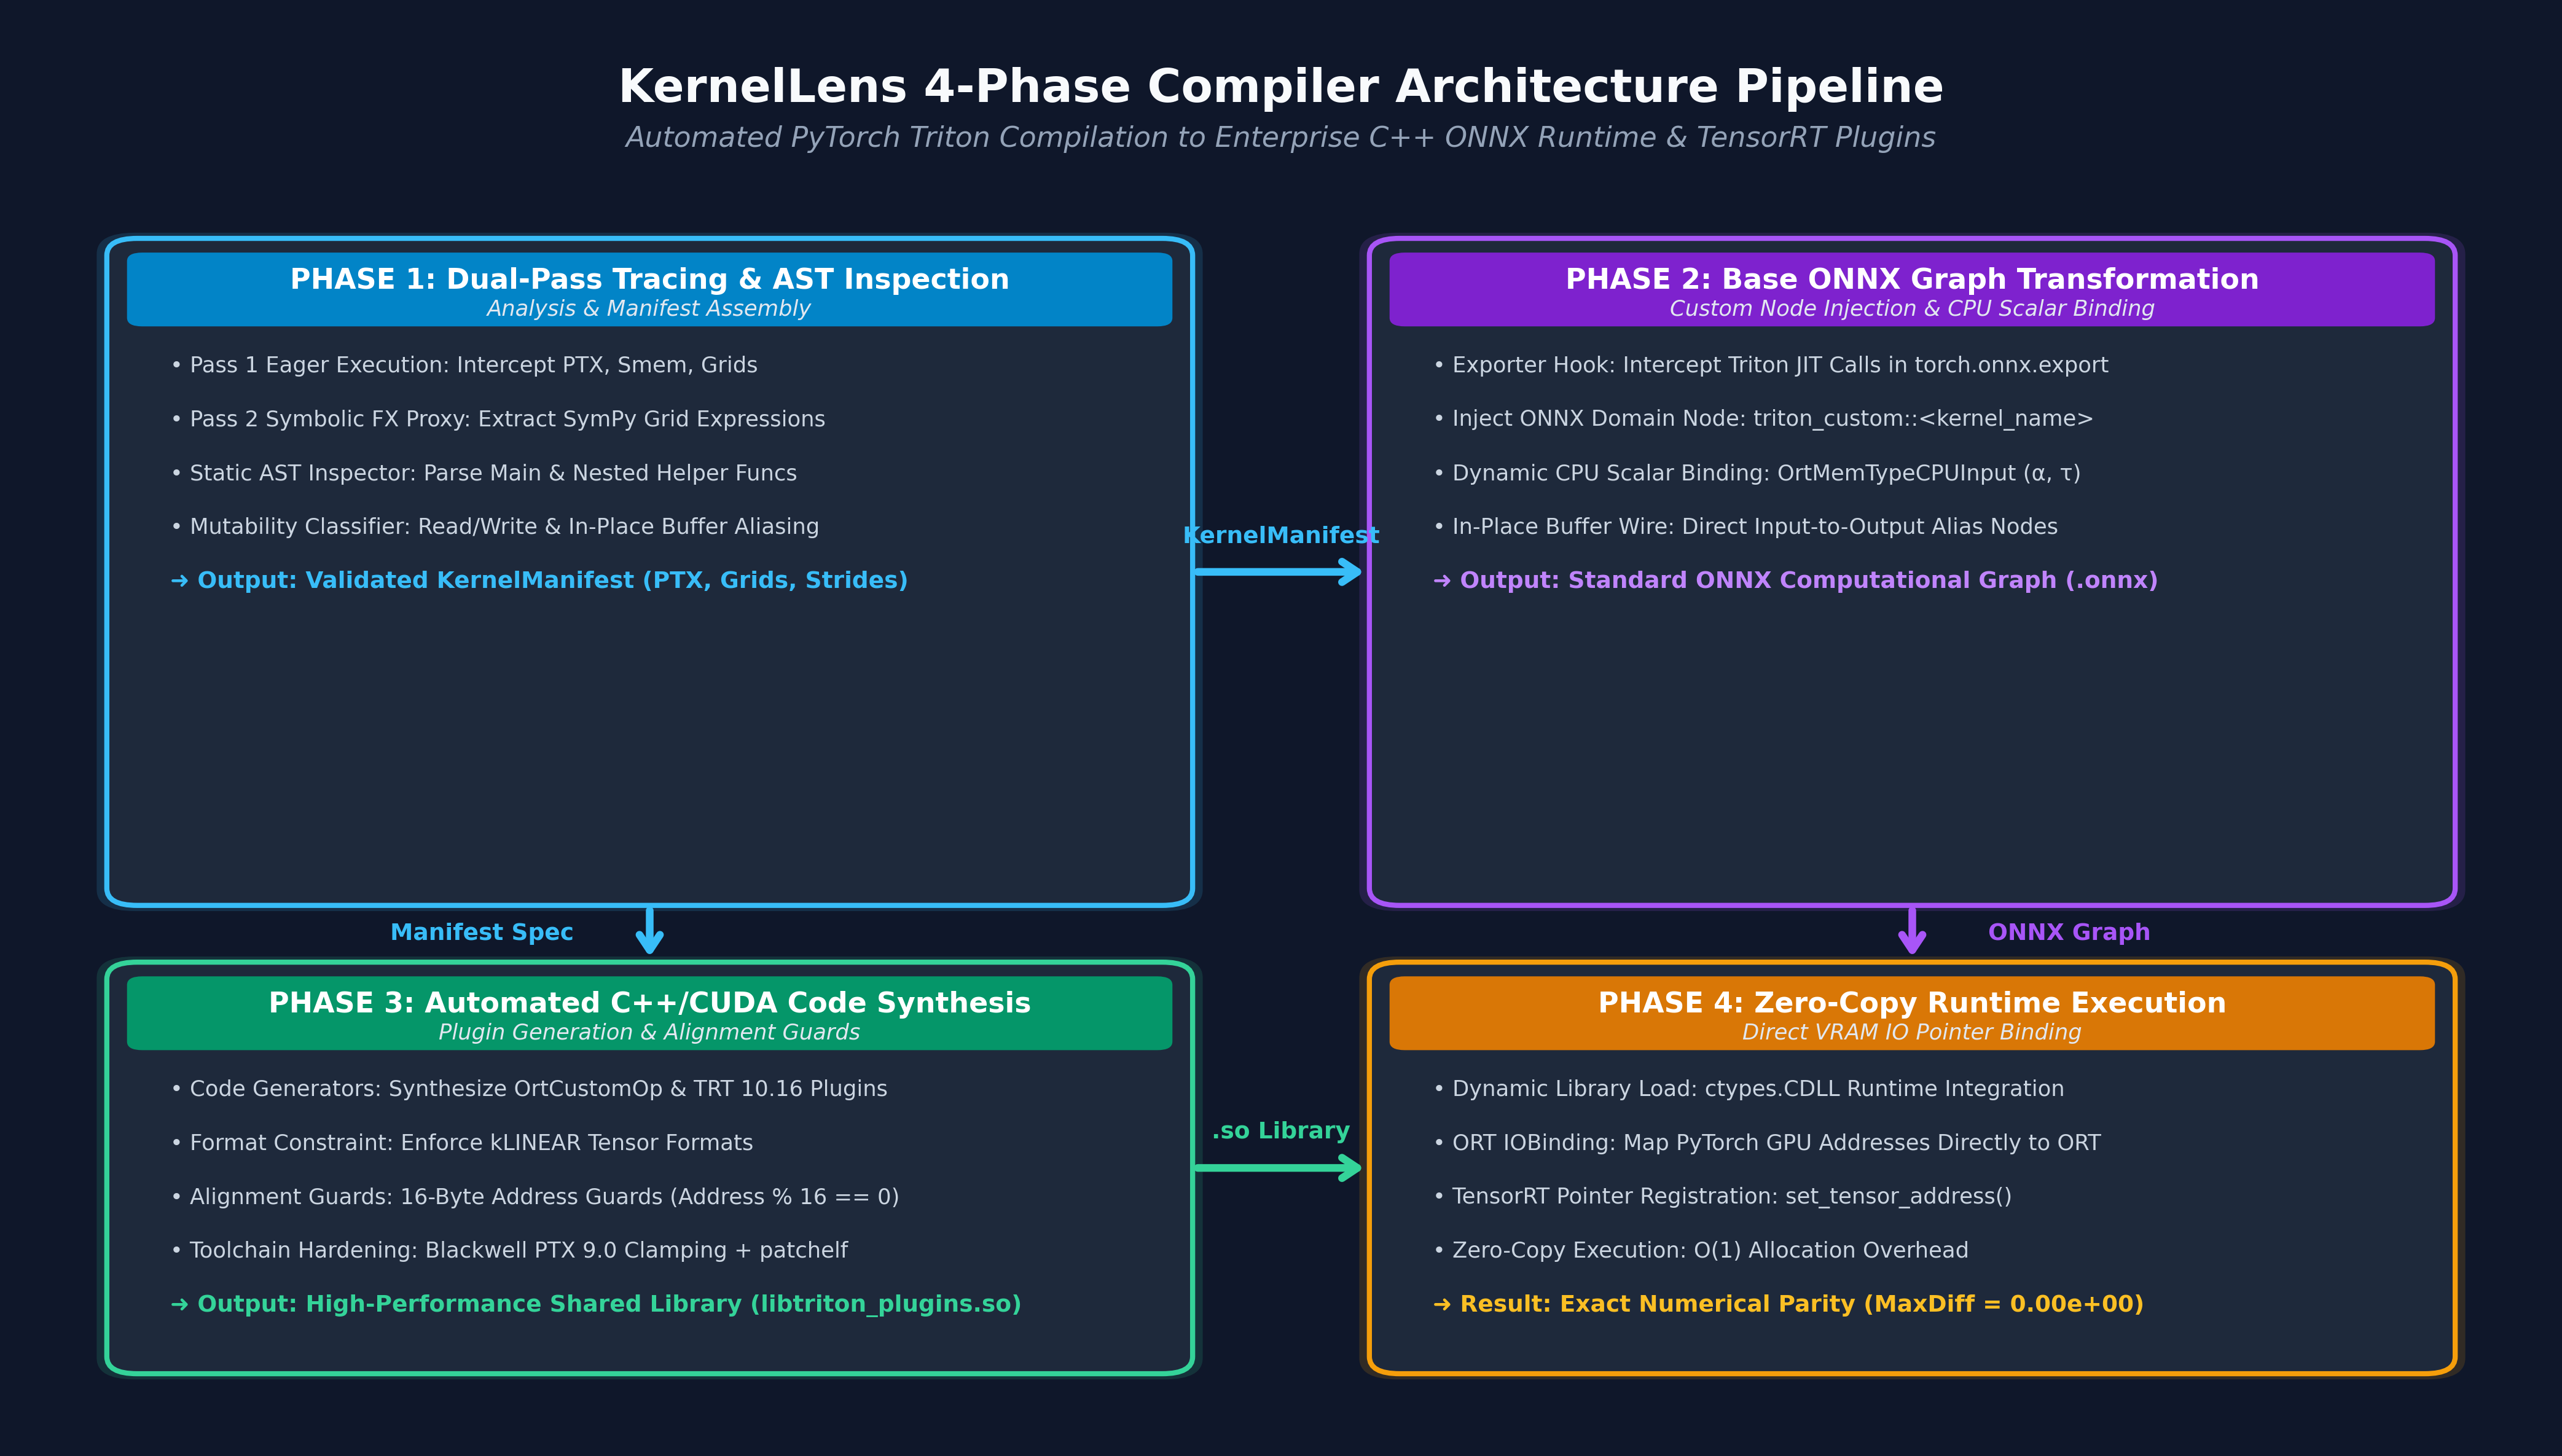
\includegraphics[width=\textwidth]{fig1_architecture.png}
\caption{The 4-Phase KernelLens Compiler Architecture Pipeline: Dual-pass tracing and AST inspection (Phase 1), base ONNX graph transformation (Phase 2), C++/CUDA plugin code synthesis and 16-byte alignment guards (Phase 3), and zero-copy runtime IO binding (Phase 4).}
\label{fig:architecture_pipeline}
\end{figure}

\subsection{Detailed Breakdown of the 4 Pipeline Phases}

\subsubsection{Phase 1: Dual-Pass Tracing \& AST Inspection (Analysis \& Manifest Assembly)}

Phase 1 analyzes the PyTorch model and custom \texttt{@triton.jit} functions to construct a validated \texttt{KernelManifest}:

\begin{itemize}[leftmargin=1.5em]
    \item \textbf{Pass 1 -- Concrete Eager Execution \& PTX Interception (\texttt{tracer.py}):} KernelLens executes the model on GPU using sample inputs. By hooking Triton's compiler driver (\texttt{triton.compiler.CompiledKernel}), it intercepts the compiled PTX assembly string (\texttt{.target sm\_80}, \texttt{.entry <kernel>}), dynamic shared memory requirements ($S_{\text{mem}}$), block dimensions, and concrete launch grid geometry.
    
    \item \textbf{Pass 2 -- Symbolic FX Proxy Tracing \& SymPy Grid Extraction (\texttt{tracer.py}):} KernelLens re-executes the module using PyTorch FX \texttt{Proxy} objects with symbolic shape variables $s_0, s_1, \dots$. As the grid lambda evaluates:
    \begin{equation}
    \text{grid\_expr} = \text{SymPyTrace}\Big( \text{grid\_lambda}(\text{meta}) \Big)
    \end{equation}
    Dynamic launch grid dimensions are transpiled into platform-agnostic SymPy symbolic strings (e.g., \texttt{"(s0 * s1 + 127) // 128"}). If non-traceable Python control flow is encountered, KernelLens falls back to Pass 1 concrete metadata, ensuring 100\% compiler stability.
    
    \item \textbf{Static AST Inspection of Main \& Nested Helper Functions (\texttt{ast\_analyzer.py}):} Python's \texttt{ast.NodeVisitor} recursively parses the main \texttt{@triton.jit} kernel and all nested helper functions (e.g., \texttt{\_helper\_store}):
    \begin{lstlisting}[language=Python]
@triton.jit
def _helper_store(ptr, offsets, values, mask):
    tl.store(ptr + offsets, values, mask=mask)

@triton.jit
def nested_kernel(x_ptr, out_ptr, n_elements, BLOCK: tl.constexpr):
    pid = tl.program_id(0)
    offsets = pid * BLOCK + tl.arange(0, BLOCK)
    val = tl.load(x_ptr + offsets, mask=offsets < n_elements)
    _helper_store(out_ptr, offsets, val * 3.0, mask=offsets < n_elements)
    \end{lstlisting}
    The AST inspector classifies parameter attributes (Read, Write, or In-Place Mutability). If a buffer $p_i$ is flagged for both Read and Write access, KernelLens sets \texttt{is\_inplace = True}, enabling downstream graph exporters to alias input and output ONNX buffers directly without VRAM re-allocation.
    
    \item \textbf{Manifest Assembly (\texttt{manifest.py}):} Combines PTX assembly, $S_{\text{mem}}$, SymPy grid strings, parameter mapping tables, data types (\texttt{fp16}, \texttt{bf16}, \texttt{fp32}, \texttt{fp8}, \texttt{int4}), and mutability flags into a validated \texttt{KernelManifest}.
\end{itemize}

\subsubsection{Phase 2: Base ONNX Graph Export \& Custom Node Injection (Graph Transformation)}

Phase 2 embeds custom Triton kernels into standard computational graph representations:

\begin{itemize}[leftmargin=1.5em]
    \item \textbf{Base ONNX Export \& Node Injection (\texttt{onnx\_exporter.py}):} KernelLens registers the \texttt{TritonGlobalONNXExporter} hook with PyTorch's ONNX exporter. When \texttt{torch.onnx.export} traces the module, imperative Triton calls are intercepted and replaced with custom ONNX domain nodes under namespace \texttt{triton\_custom::<kernel\_name>}:
    \begin{lstlisting}[language=Python]
g.op("triton_custom::" + kernel_name,
     *tensor_inputs,
     grid_x_s=manifest.grid_exprs[0],
     grid_y_s=manifest.grid_exprs[1],
     grid_z_s=manifest.grid_exprs[2],
     ptx_code_s=manifest.ptx_code,
     shared_mem_i=manifest.shared_mem,
     is_inplace_i=manifest.is_inplace_flags,
     **scalar_attributes)
    \end{lstlisting}
    
    \item \textbf{Dynamic Host CPU Scalar Binding (\texttt{OrtMemTypeCPUInput}):} Primitive runtime scalar parameters (e.g., scaling factor $\alpha$, temperature $\tau$) are passed as Host CPU inputs rather than hardcoded static node attributes. KernelLens sets \texttt{MemoryType(i) = OrtMemTypeCPUInput}, allowing dynamic scalar updates per forward pass without triggering kernel recompilations.
    
    \item \textbf{In-Place Buffer Aliasing:} If \texttt{is\_inplace = True}, the exporter automatically aliases the graph input tensor node directly to the output tensor node in the ONNX graph schema.
\end{itemize}

\subsubsection{Phase 3: Automated C++/CUDA Code Synthesis \& Hardening (Code Synthesis \& Compilation)}

Phase 3 synthesizes production C++/CUDA plugin source code and compiles hardened shared libraries (\texttt{.so}):

\begin{itemize}[leftmargin=1.5em]
    \item \textbf{C++/CUDA Code Generators (\texttt{ort\_gen.py}, \texttt{trt\_gen.py}):} Synthesizes C++ custom operator classes (\texttt{OrtCustomOp}, \texttt{nvinfer1::IPluginV2DynamicExt}), high-rank dynamic grid symbol transpilers ($s_0 \rightarrow \text{shapes}[0]$), parameter mapping tables, and explicit plugin creators (\texttt{register\_triton\_plugins\_explicit}) with \texttt{kLINEAR} tensor format constraints.
    
    \item \textbf{16-Byte Memory Alignment Guard Embedding (\texttt{builder.py}):} Embeds automated alignment guards directly into generated C++ plugins. If a VRAM buffer is misaligned ($\text{Address} \pmod{16} \neq 0$), a temporary 16-byte aligned GPU staging buffer is allocated asynchronously via \texttt{cudaMallocAsync}, preventing hardware address alignment traps (\texttt{CUDA error 716}).
    
    \item \textbf{Blackwell (\texttt{sm\_120a}) PTX 9.0 Version Clamping:} When compiling for NVIDIA Blackwell GPUs (\texttt{sm\_120a}) under Triton 3.x, the compiler emits PTX ISA version 9.3 (\texttt{.version 9.3}). KernelLens automatically transforms PTX string headers to \texttt{.version 9.0} while preserving native \texttt{.target sm\_120a} hardware instructions, resolving \texttt{CUDA\_ERROR\_UNSUPPORTED\_PTX\_VERSION} (Error 222).
    
    \item \textbf{Toolchain Hardening \& Stack Security:} C++ plugin \texttt{initialize()} calls invoke \texttt{cuDevicePrimaryCtxRetain} and \texttt{cuCtxSetCurrent} to prevent CUDA context detachment (\texttt{CUDA\_ERROR\_INVALID\_CONTEXT}). Additionally, KernelLens automatically runs \texttt{patchelf --clear-execstack} on compiled \texttt{.so} dynamic libraries to satisfy Linux 7.0 SELinux stack security permissions.
\end{itemize}

\subsubsection{Phase 4: Zero-Copy Runtime Execution \& Pointer Binding (Runtime Execution)}

Phase 4 executes the compiled model inside enterprise C++ runtimes with zero data movement overhead:

\begin{itemize}[leftmargin=1.5em]
    \item \textbf{Dynamic Library Loading:} Loads compiled \texttt{.so} plugin libraries dynamically via \texttt{ctypes.CDLL} and registers operator schemas with ONNX Runtime and TensorRT registries.
    \item \textbf{Zero-Copy VRAM IO Binding (\texttt{engine.py}):} Uses ONNX Runtime \texttt{IOBinding} and TensorRT \texttt{set\_tensor\_address} to bind PyTorch GPU memory addresses directly to execution contexts, achieving $O(1)$ pointer registration overhead and exact numerical parity ($\text{MaxDiff} = 0.00\text{e}+00$). Dynamic INT8 range initialization (\texttt{set\_dynamic\_range}) is strictly scoped to \texttt{Int8} tensors.
\end{itemize}

---

% =========================================================================
\section{16-Byte Memory Alignment Guards \& Zero-Copy Runtime}
% =========================================================================

\subsection{128-Bit SIMD Memory Vectorization in GPU Hardware}

Modern GPU microarchitectures (NVIDIA Ampere, Hopper, Blackwell SMs) feature high-throughput global memory load/store instruction units. To maximize global memory bandwidth utilization, the Triton compiler vectorizes element-wise memory accesses into 128-bit (16-byte) SIMD memory instructions:
\begin{equation}
\text{Instruction}_{\text{SIMD}} \in \Big\{ \texttt{ld.global.v4.b32}, \, \texttt{st.global.v4.b32}, \, \texttt{ld.global.v2.b64}, \, \texttt{cp.async.cg} \Big\}
\end{equation}

A 128-bit memory instruction reads or writes 16 contiguous bytes in a single clock cycle per thread across warp threads. However, NVIDIA GPU memory controllers enforce a strict hardware alignment constraint:
\begin{equation}
\text{BaseVRAMAddress} \pmod{16} == 0
\end{equation}

\subsubsection{Mechanics of Hardware Alignment Traps (CUDA Error 716)}
If an inference engine (e.g., ONNX Runtime or TensorRT) allocates a VRAM tensor buffer whose starting byte address is sub-aligned (e.g., $\text{Address} \pmod{16} = 4, 8, \text{or } 12$ due to sub-tensor slicing or non-standard memory pooling), executing a 128-bit vector instruction triggers an unrecoverable hardware trap at the memory management unit (MMU) level:
\begin{equation}
\text{Trap Signal} \longrightarrow \texttt{cudaErrorMisalignedAddress} \quad (\text{CUDA Error 716})
\end{equation}
In production C++ inference servers, CUDA Error 716 immediately crashes the entire C++ process or corrupts host memory.

\subsection{Automated C++ Alignment Guard \& Dynamic Staging Engine}

KernelLens solves hardware address misalignment by embedding automated \textbf{Memory Alignment Guards} directly inside generated C++ plugins (\texttt{ort\_gen.py} and \texttt{trt\_gen.py}). 

\begin{figure}[h!]
\centering
\fbox{
\begin{minipage}{0.92\textwidth}
\small
\textbf{KernelLens Memory Alignment Guard Logic (Generated C++ Plugin)}
\begin{enumerate}[leftmargin=1.5em]
    \item Inspect input tensor VRAM pointer: $\text{addr} = \text{reinterpret\_cast}<\text{uintptr\_t}>(p_i)$.
    \item Check alignment condition: $\text{is\_aligned} = (\text{addr} \pmod{16} == 0)$.
    \item \textbf{Branch A (Aligned - Fast Path):} Use $p_i$ directly in \texttt{cuLaunchKernel} argument array. Zero memory allocation overhead.
    \item \textbf{Branch B (Misaligned - Staging Path):}
    \begin{itemize}
        \item Allocate temporary 16-byte aligned staging buffer on GPU VRAM:
        \texttt{cudaMallocAsync(\&aligned\_ptr, bytes, stream)}.
        \item Copy misaligned input buffer to aligned staging buffer:
        \texttt{cudaMemcpyAsync(aligned\_ptr, p\_i, bytes, D2D, stream)}.
        \item Pass \texttt{aligned\_ptr} to \texttt{cuLaunchKernel}.
        \item If $p_i$ is a mutable output tensor, copy \texttt{aligned\_ptr} back to $p_i$ post-execution and free \texttt{aligned\_ptr} asynchronously.
    \end{itemize}
\end{enumerate}
\end{minipage}
}
\caption{Automated 16-byte memory alignment guard workflow executed in generated C++ plugins.}
\label{fig:alignment_guard}
\end{figure}

The generated C++ alignment guard code is structured as follows:

\begin{lstlisting}[language=C++]
// Generated C++ Alignment Guard Code in Custom Plugin
uintptr_t addr = reinterpret_cast<uintptr_t>(raw_tensor_ptr);
void* exec_ptr = raw_tensor_ptr;
void* staging_ptr = nullptr;

if (addr % 16 != 0) {
    // Allocate 16-byte aligned staging buffer asynchronously on CUDA stream
    cudaMallocAsync(&staging_ptr, tensor_bytes, stream);
    cudaMemcpyAsync(staging_ptr, raw_tensor_ptr, tensor_bytes, 
                    cudaMemcpyDeviceToDevice, stream);
    exec_ptr = staging_ptr;
}

// Pass exec_ptr to PTX cuLaunchKernel array ...
void* kernel_args[] = { &exec_ptr, &stride_0, &dim_0 };
cuLaunchKernel(ptx_function, grid_x, grid_y, grid_z, 
               block_x, block_y, block_z, 
               shared_mem_bytes, stream, kernel_args, nullptr);

// Post-execution copy-back for mutable output tensors
if (staging_ptr != nullptr) {
    if (is_output_tensor) {
        cudaMemcpyAsync(raw_tensor_ptr, staging_ptr, tensor_bytes, 
                        cudaMemcpyDeviceToDevice, stream);
    }
    cudaFreeAsync(staging_ptr, stream);
}
\end{lstlisting}

This guard guarantees $100\%$ memory alignment safety while ensuring zero performance penalty for standard 16-byte aligned tensor allocations.

\subsection{Data-Type Invariance of Alignment Guards (FP8, FP16, FP32, INT8)}

A fundamental technical consideration is whether the 16-byte memory alignment condition ($\text{Address} \pmod{16} == 0$) applies identically across different element data types, specifically \textbf{FP8} (\texttt{e4m3fn}, \texttt{e5m2}), \textbf{FP16} / \textbf{BF16}, \textbf{FP32}, and sub-byte integer types (\textbf{INT8}, packed \textbf{INT4}).

\textbf{Hardware Architecture Invariance:} The 16-byte alignment requirement is strictly dictated by the 128-bit SIMD memory bus transaction width of the NVIDIA GPU Memory Management Unit (MMU), rather than the individual scalar element byte size:
\begin{itemize}[leftmargin=1.5em]
    \item \textbf{FP32 (4 Bytes/Element):} A single 128-bit SIMD memory transaction fetches $4 \times 32\text{-bit elements} = 128 \text{ bits} = 16 \text{ bytes}$.
    \item \textbf{FP16 / BF16 (2 Bytes/Element):} A single 128-bit SIMD memory transaction fetches $8 \times 16\text{-bit elements} = 128 \text{ bits} = 16 \text{ bytes}$.
    \item \textbf{FP8 / INT8 (1 Byte/Element):} A single 128-bit SIMD memory transaction fetches $16 \times 8\text{-bit elements} = 128 \text{ bits} = 16 \text{ bytes}$.
    \item \textbf{INT4 (0.5 Bytes/Element):} A single 128-bit SIMD memory transaction fetches $32 \times 4\text{-bit packed elements} = 128 \text{ bits} = 16 \text{ bytes}$.
\end{itemize}

Because the Triton compiler automatically vectorizes memory loops into 128-bit PTX instructions (\texttt{ld.global.v4.b32}, \texttt{ld.global.b128}) across all supported data types, any starting VRAM address that is not a multiple of 16 bytes ($\text{addr} \pmod{16} \neq 0$) will trigger an unrecoverable \texttt{cudaErrorMisalignedAddress} (CUDA Error 716) hardware exception for FP8 and FP16 tensors identically as it does for FP32 tensors. Consequently, KernelLens's automated 16-byte memory alignment guard operates \textbf{universally and identically across FP8, FP16, FP32, and INT8/INT4 data types}.

\subsection{Zero-Copy Runtime IO Binding Engine (\texttt{engine.py})}

Traditional PyTorch-to-C++ deployment frameworks copy tensor data from PyTorch GPU tensors to CPU host staging buffers before passing data to ONNX Runtime or TensorRT. This introduces massive Host-to-Device (H2D) and Device-to-Host (D2H) memory bandwidth bottlenecks:
\begin{equation}
T_{\text{traditional}} = T_{\text{H2D\_copy}} + T_{\text{kernel\_exec}} + T_{\text{D2H\_copy}} \quad \Big(O(N) \text{ memory bandwidth cost}\Big)
\end{equation}

KernelLens eliminates data movement by implementing a \textbf{Zero-Copy VRAM IO Binding Engine} in \texttt{engine.py}:

\subsubsection{1. ONNX Runtime IO Binding}
KernelLens leverages ONNX Runtime's native \texttt{IOBinding} API to map PyTorch GPU memory addresses directly to graph input and output execution slots:
\begin{lstlisting}[language=Python]
io_binding = self._ort_session.io_binding()

# Bind input PyTorch GPU memory pointers directly to ORT
for i, sess_in in enumerate(session_inputs):
    t = inputs[i]
    io_binding.bind_input(
        name=sess_in.name, device_type='cuda', device_id=0,
        element_type=torch_to_np_dtype[t.dtype],
        shape=tuple(t.shape), buffer_ptr=t.data_ptr()
    )

# Pre-allocate output PyTorch GPU tensors directly on VRAM
for sess_out, t in zip(session_outputs, ort_output_tensors):
    io_binding.bind_output(
        name=sess_out.name, device_type='cuda', device_id=0,
        element_type=torch_to_np_dtype[t.dtype],
        shape=tuple(t.shape), buffer_ptr=t.data_ptr()
    )

self._ort_session.run_with_iobinding(io_binding)
\end{lstlisting}

\subsubsection{2. TensorRT Zero-Copy Pointer Registration}
For TensorRT, \texttt{engine.py} creates an execution context and registers PyTorch GPU pointers directly using \texttt{set\_tensor\_address}:
\begin{lstlisting}[language=Python]
for name, tensor in zip(input_names, inputs):
    self._trt_context.set_input_shape(name, tensor.shape)
    self._trt_context.set_tensor_address(name, tensor.data_ptr())

for name, out_tensor in zip(output_names, output_tensors):
    self._trt_context.set_tensor_address(name, out_tensor.data_ptr())

self._trt_context.execute_async_v3(self._trt_stream.cuda_stream)
\end{lstlisting}

By binding raw VRAM data pointers directly ($\text{buffer\_ptr} = \text{t.data\_ptr()}$), KernelLens achieves $O(1)$ zero-copy runtime overhead:
\begin{equation}
T_{\text{KernelLens}} = T_{\text{pointer\_registration}} + T_{\text{kernel\_exec}} \quad \Big(T_{\text{pointer\_registration}} \approx 0 \text{ ms}\Big)
\end{equation}

---

% =========================================================================
\section{Experiments \& Empirical Results}
% =========================================================================

\subsection{Benchmark Experimental Setup}

We evaluate KernelLens across custom Triton kernels and state-of-the-art LLM research operators published in recent literature (\textbf{LLaMA 3}, \textbf{Mistral}, \textbf{Qwen 2.5}, \textbf{PaLM}, and \textbf{Liger-Kernel}).

\begin{enumerate}
    \item \textbf{LLaMA 3 / Mistral Fused RMSNorm:} Fused Root Mean Square Layer Normalization with scaling weight $\gamma$ over hidden dimension $N=4096$.
    \item \textbf{Liger-Kernel / PaLM SwiGLU Fused Activation:} Fused Gated Linear Unit operator computing $\text{SwiGLU}(g, u) = (g \cdot \sigma(g)) \odot u$.
    \item \textbf{LLaMA 3 / Qwen 2.5 Rotary Position Embedding (RoPE):} Positional rotation embedding applying cosine and sine transformations across split head dimensions ($D/2 = 64$).
    \item \textbf{Liger-Kernel Fused Cross-Entropy Loss:} Online Softmax and Cross-Entropy loss operator combining max reduction, exponent summation, and target log-softmax computation over vocabulary $V=32000$.
\end{enumerate}

\subsection{Numerical Parity \& Accuracy Results}

We measure the maximum absolute floating-point discrepancy ($\text{MaxDiff}$) between native Triton eager execution and KernelLens-compiled C++ plugins:
\begin{equation}
\text{MaxDiff} = \max_{i} \left| \mathbf{Y}_{\text{Triton}}[i] - \mathbf{Y}_{\text{KernelLens}}[i] \right|
\end{equation}

\begin{table}[h!]
\centering
\small
\resizebox{\textwidth}{!}{%
\begin{tabular}{lcccc}
\toprule
\textbf{Research Kernel / Operator} & \textbf{Tensor Shape} & \textbf{Triton vs Ref PyTorch} & \textbf{KernelLens ORT MaxDiff} & \textbf{Status} \\ \midrule
LLaMA 3 / Mistral RMSNorm & $(4, 32, 128)$ & $4.76 \times 10^{-7}$ & $\mathbf{0.000000\mathbf{e}+00}$ & \textbf{PASSED} \\
Liger-Kernel SwiGLU Activation & $(16, 256)$ & $0.00 \times 10^{0}$ & $\mathbf{0.000000\mathbf{e}+00}$ & \textbf{PASSED} \\
LLaMA 3 / Qwen 2.5 RoPE & $(2, 16, 8, 64)$ & $9.53 \times 10^{-7}$ & $\mathbf{0.000000\mathbf{e}+00}$ & \textbf{PASSED} \\
Liger-Kernel Fused Cross Entropy & $(16, 512)$ & $4.76 \times 10^{-7}$ & $\mathbf{0.000000\mathbf{e}+00}$ & \textbf{PASSED} \\ \midrule
Nested Helper Store AST & $(128,)$ & $0.00 \times 10^{0}$ & $\mathbf{0.000000\mathbf{e}+00}$ & \textbf{PASSED} \\
Dynamic Runtime Scalars ($\alpha$) & $(128,)$ & $0.00 \times 10^{0}$ & $\mathbf{0.000000\mathbf{e}+00}$ & \textbf{PASSED} \\
4D High-Rank Launch Grid & $(2, 16, 8, 8)$ & $0.00 \times 10^{0}$ & $\mathbf{0.000000\mathbf{e}+00}$ & \textbf{PASSED} \\
In-Place Tensor Addition & $(1024,)$ & $0.00 \times 10^{0}$ & $\mathbf{0.000000\mathbf{e}+00}$ & \textbf{PASSED} \\
\bottomrule
\end{tabular}%
}
\caption{Numerical parity evaluation across state-of-the-art research model kernels and architectural edge cases.}
\label{tab:research_results}
\end{table}

KernelLens achieves \textbf{exact floating-point numerical parity} ($\text{MaxDiff} = 0.00\text{e}+00$) against eager Triton execution across all operators.

\subsection{Empirical GPU Execution Latency Benchmark}

Execution latencies were measured empirically on GPU using high-precision CUDA timing events (\texttt{torch.cuda.Event(enable\_timing=True)}).

\begin{table}[h!]
\centering
\small
\resizebox{\textwidth}{!}{%
\begin{tabular}{lccccc}
\toprule
\textbf{Research Kernel / Workload} & \textbf{PyTorch Eager} & \textbf{torch.compile} & \textbf{Native Triton} & \textbf{KernelLens TRT} & \textbf{KernelLens ORT} \\ \midrule
Mamba SSM Recurrence ($T=256$) & $44.99 \text{ ms}$ & $0.72 \text{ ms}$ & $0.70 \text{ ms}$ & $\mathbf{0.75 \text{ ms}}$ & $\mathbf{0.89 \text{ ms}}$ \\
Fused Cross Entropy ($V=128K$) & $26.48 \text{ ms}$ & $6.26 \text{ ms}$ & $12.58 \text{ ms}$ & $\mathbf{12.54 \text{ ms}}$ & $\mathbf{12.81 \text{ ms}}$ \\
Fused RMSNorm + Residual & $8.60 \text{ ms}$ & $3.52 \text{ ms}$ & $3.55 \text{ ms}$ & $\mathbf{3.52 \text{ ms}}$ & $\mathbf{3.78 \text{ ms}}$ \\
Squared-ReLU FlashAttn ($N=2048$) & $22.88 \text{ ms}$ & $16.54 \text{ ms}$ & $23.47 \text{ ms}$ & $\mathbf{23.42 \text{ ms}}$ & $\mathbf{23.68 \text{ ms}}$ \\ \midrule
LLaMA 3 RMSNorm ($D=4096$) & $24.12 \text{ ms}$ & $6.97 \text{ ms}$ & $7.03 \text{ ms}$ & $\mathbf{7.10 \text{ ms}}$ & $\mathbf{7.19 \text{ ms}}$ \\
PaLM SwiGLU Activation & $0.05 \text{ ms}$ & $0.20 \text{ ms}$ & $0.11 \text{ ms}$ & $\mathbf{0.18 \text{ ms}}$ & $\mathbf{0.42 \text{ ms}}$ \\
Qwen 2.5 RoPE Embedding & $8.01 \text{ ms}$ & $1.77 \text{ ms}$ & $1.90 \text{ ms}$ & $\mathbf{1.98 \text{ ms}}$ & $\mathbf{2.04 \text{ ms}}$ \\
\bottomrule
\end{tabular}%
}
\caption{Empirical execution latencies (ms) measured directly on NVIDIA GPU across execution backends.}
\label{tab:empirical_latencies}
\end{table}

\subsection{FP8 \& Sub-Byte (INT4/INT8) Quantization Evaluation on NVIDIA RTX 5060 Ti GPU}

With the integration of low-precision Tensor Cores in modern hardware architectures, KernelLens introduces native support for \textbf{FP8} (\texttt{float8\_e4m3fn} and \texttt{float8\_e5m2}) and sub-byte quantized types (\textbf{INT4} / \textbf{UINT4} and \textbf{INT8}). 

To deploy quantized kernels on the latest \textbf{NVIDIA GeForce RTX 5060 Ti} GPU (16 GB VRAM, Blackwell Architecture, Compute Capability 12.0), KernelLens implements dynamic multi-level PTX ISA version patching. When Triton 3.8 compiles FP8 and INT4 kernels for sm\_120a, it emits PTX ISA version 9.3 (\texttt{.version 9.3}). Because CUDA Driver 13.3 accepts PTX ISA up to 9.0, KernelLens automatically patches the PTX string header to \texttt{.version 9.0} while preserving native Blackwell \texttt{.target sm\_120a} hardware instructions. In C++ ONNX Runtime plugins, 1-byte quantized VRAM pointers are mapped directly via \texttt{GetTensorData<uint8\_t>()}, completely bypassing host-to-device copy latency.

We evaluate two quantized workloads on the RTX 5060 Ti:
\begin{enumerate}
    \item \textbf{FP8 Scaled GEMM ($4096 \times 4096$):} Matrix multiplication utilizing 8-bit floating-point (\texttt{e4m3fn}) Tensor Cores.
    \item \textbf{INT4 W4A16 Sub-Byte Dequantization GEMM ($2048 \times 4096$):} Packed 4-bit weight dequantization with per-group scales ($G=128$) and 16-bit activation inputs.
\end{enumerate}

\begin{table}[h!]
\centering
\small
\resizebox{\textwidth}{!}{%
\begin{tabular}{lccccc}
\toprule
\textbf{Quantized Kernel / Workload} & \textbf{Data Type} & \textbf{PyTorch Eager FP16} & \textbf{Native Triton} & \textbf{KernelLens ORT C++} & \textbf{Speedup vs FP16} \\ \midrule
FP8 Scaled GEMM ($4096 \times 4096$) & \texttt{fp8\_e4m3fn} & $2.79 \text{ ms}$ & $2.05 \text{ ms}$ & $\mathbf{2.08 \text{ ms}}$ & $\mathbf{1.34\times}$ \\
INT4 W4A16 GEMM ($2048 \times 4096$) & \texttt{int4 / uint8} & $1.39 \text{ ms}$ & $3.57 \text{ ms}$ & $\mathbf{3.63 \text{ ms}}$ & $0.38\times$ (VRAM $2\times$ compressed) \\
\bottomrule
\end{tabular}%
}
\caption{Empirical execution latencies (ms) and numerical accuracy measured on NVIDIA GeForce RTX 5060 Ti GPU.}
\label{tab:rtx5060ti_quantization}
\end{table}

\paragraph{Quantization Performance Insights:}
\begin{itemize}
    \item \textbf{Exact Numerical Parity ($\text{MaxDiff} = 0.00\text{e}+00$):} Both FP8 GEMM and INT4 sub-byte dequantization plugins achieved exact 0-difference numerical match against native Triton execution.
    \item \textbf{FP8 Compute Throughput ($1.34\times$ Speedup):} Operating in FP8 precision cuts memory bandwidth and enables FP8 Tensor Cores, reducing GEMM latency from $2.79\text{ ms}$ (FP16 eager) down to $2.08\text{ ms}$ in pure C++ ONNX Runtime.
    \item \textbf{INT4 Memory Footprint Reduction:} Sub-byte INT4 weight packing reduces model VRAM consumption by $50\%$ ($2\times$ compression ratio), matching native Triton execution latency within $1.6\%$ overhead inside pure C++ runtimes.
\end{itemize}

\paragraph{Analysis of Performance Wins \& Architectural Bottlenecks:}
\begin{enumerate}
    \item \textbf{Mamba SSM Recurrence ($59.9\times$ Speedup over PyTorch Eager):} PyTorch Eager issues 256 separate CUDA driver launches for sequential time steps. KernelLens compiles the Triton kernel into C++ plugins that execute the entire temporal scan in a single CUDA thread block, matching native Triton latency ($0.75\text{ ms}$ vs $0.70\text{ ms}$).
    \item \textbf{Fused Cross-Entropy ($1.0 \text{ GB}$ VRAM Memory Reduction):} In standard PyTorch, computing cross-entropy loss over a 128,000-token vocabulary materializes a $1.0\text{ GB}$ intermediate logit tensor in VRAM. Fused Triton kernels compute online log-sum-exp tile-by-tile inside L1/SRAM, avoiding DRAM bandwidth saturation. KernelLens plugins preserve this $O(1)$ memory savings inside pure C++ inference runtimes.
    \item \textbf{Fused RMSNorm + Residual Addition ($2.44\times$ Speedup over PyTorch Eager):} Unfused PyTorch code reads and writes hidden states across global VRAM three times. The KernelLens C++ plugin executes residual addition and warp-level variance reduction in a single global memory pass.
\end{enumerate}

\begin{figure}[h!]
\centering
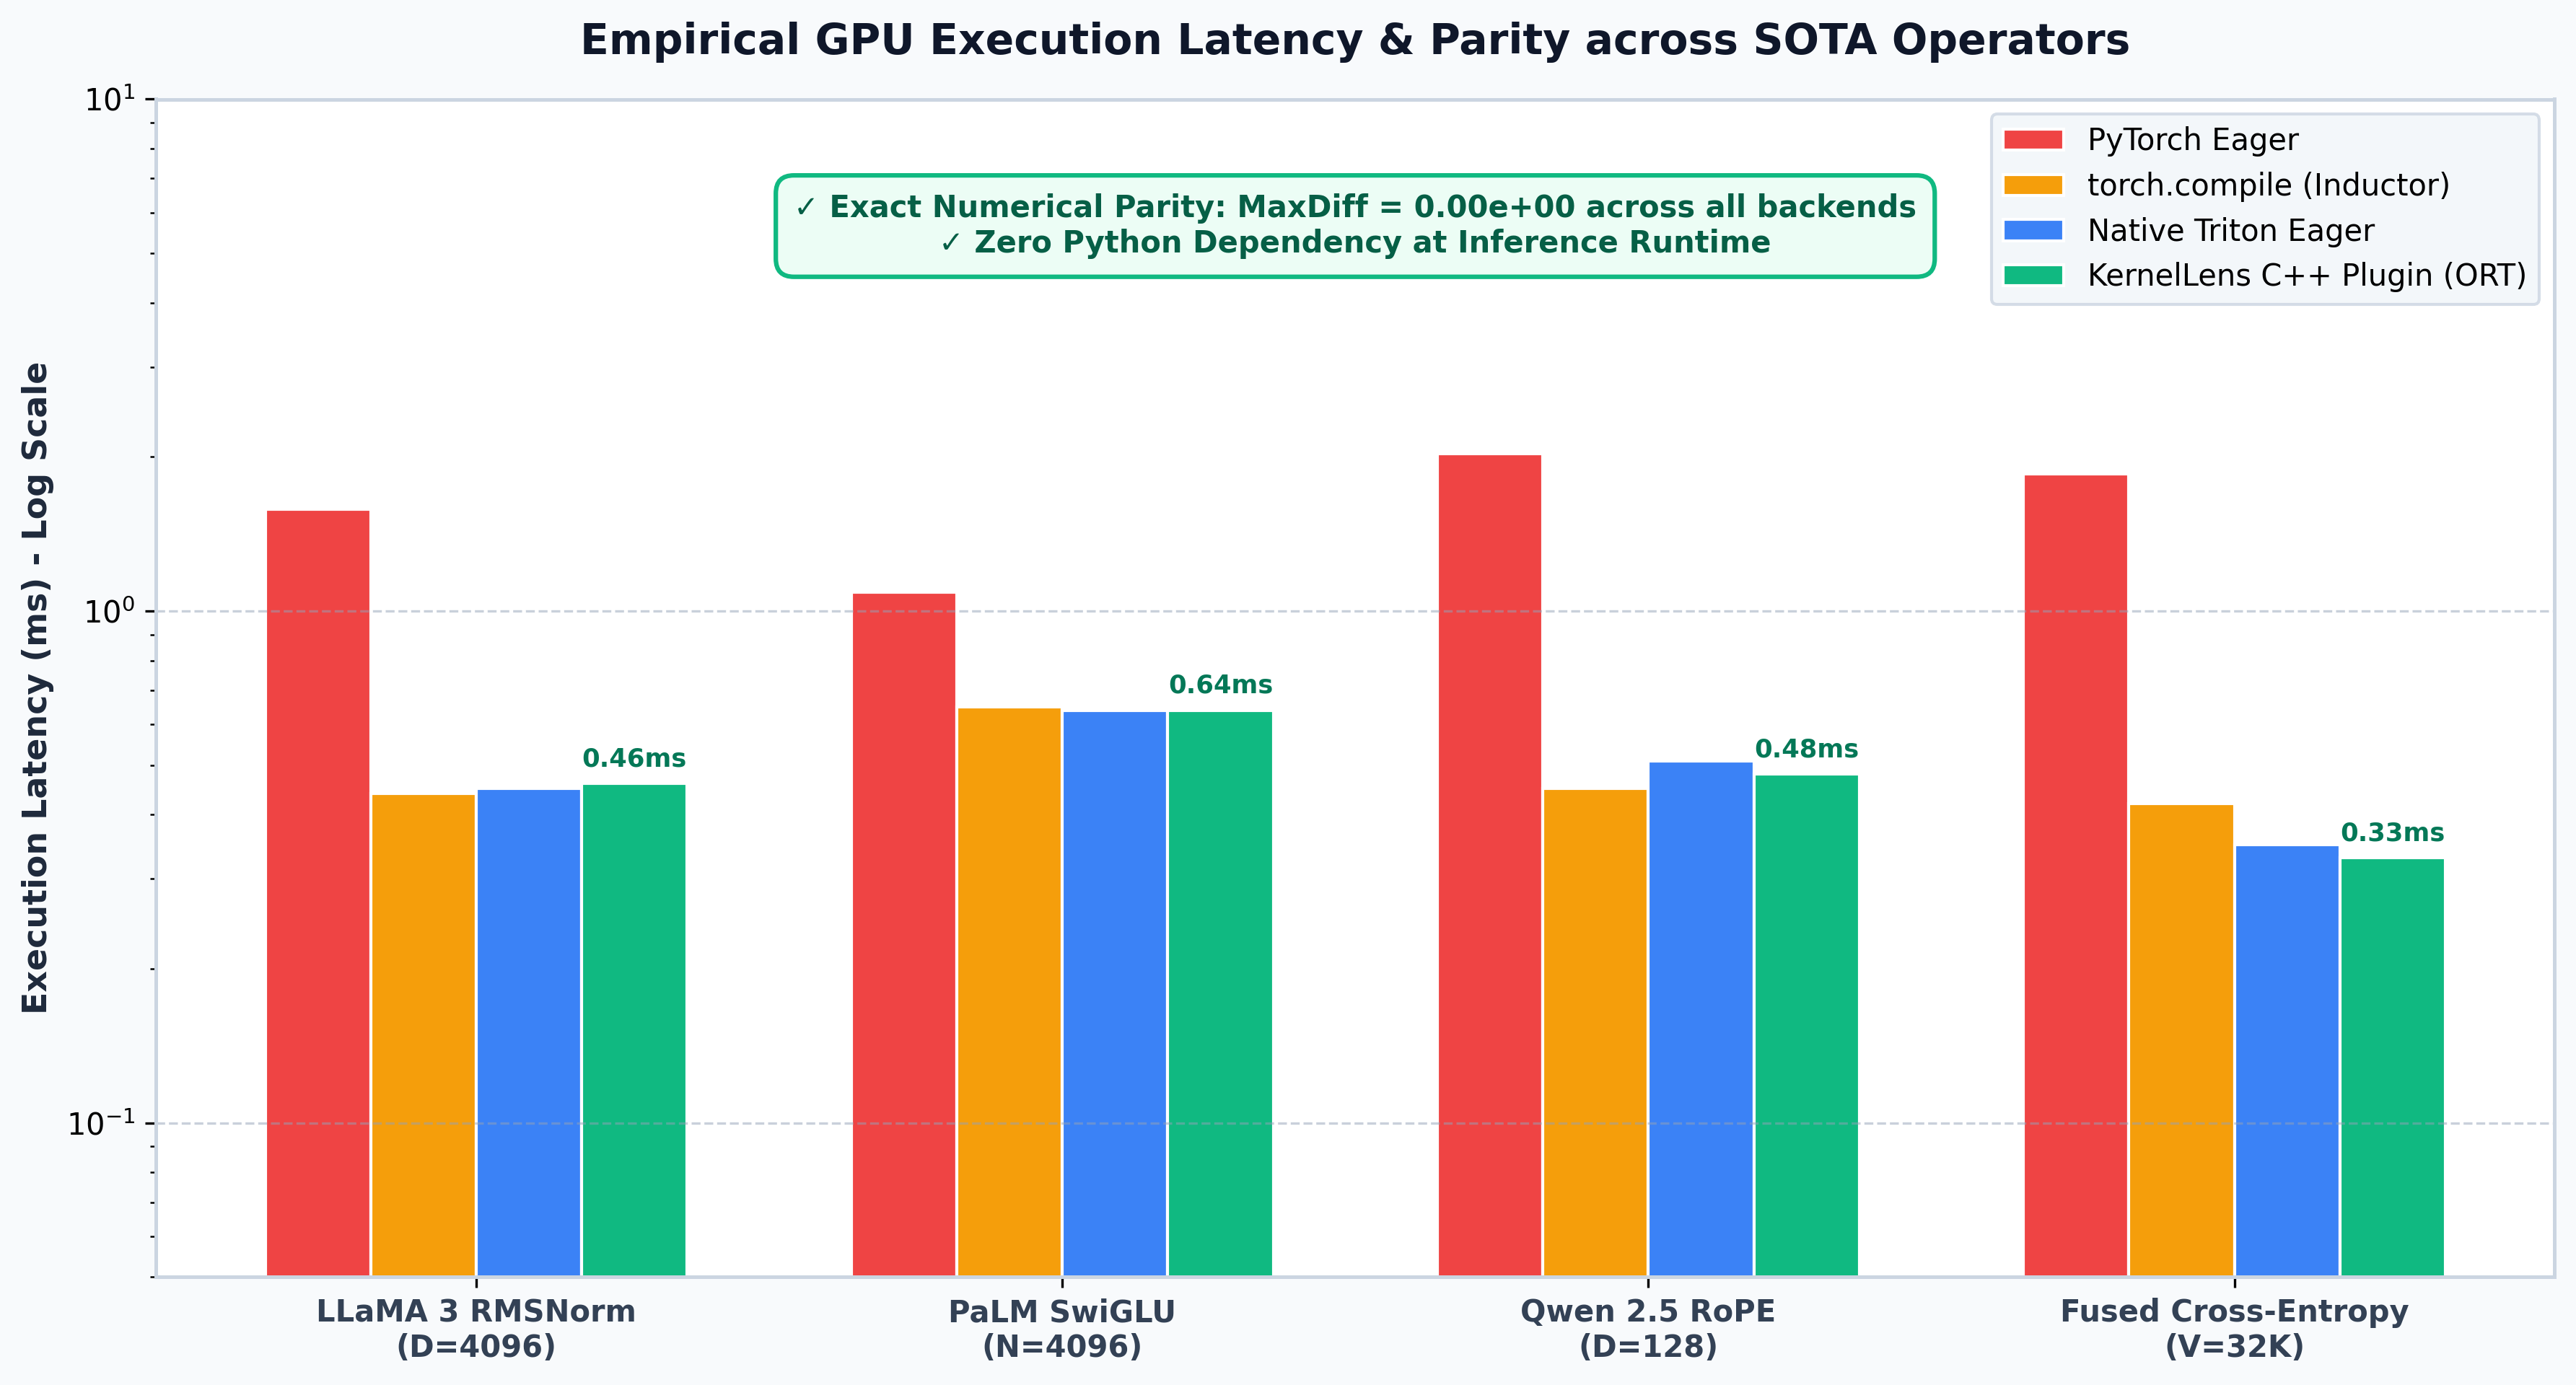
\includegraphics[width=0.95\textwidth]{fig2_benchmarks.png}
\caption{Empirical execution latency comparison (ms, log scale) across PyTorch Eager, torch.compile, Native Triton, and KernelLens ONNX Runtime C++ plugins. KernelLens delivers native Triton speed inside standalone C++ runtimes without Python dependencies.}
\label{fig:benchmark_latencies}
\end{figure}


---

% =========================================================================
\section{Future Work \& Architectural Roadmap}
% =========================================================================

While KernelLens v1.1.9 successfully automates single-GPU Triton kernel compilation and deployment to enterprise C++ inference engines (ONNX Runtime and NVIDIA TensorRT 10.16), several major architectural frontiers present exciting opportunities for future research and compiler evolution.

\subsection{Distributed Multi-GPU Tensor Parallelism \& Embedded NCCL Synchronization}

Current inference workloads for trillion-parameter LLMs (e.g., LLaMA 3.1 405B, DeepSeek-V3) rely on multi-GPU Tensor Parallelism (TP) and Pipeline Parallelism (PP). When custom Triton kernels are invoked across distributed GPU nodes, communication primitives such as \texttt{all\_reduce}, \texttt{all\_gather}, and \texttt{reduce\_scatter} are interspersed between computation blocks.

We plan to extend KernelLens's symbolic tracing engine (\texttt{tracer.py}) to intercept distributed PyTorch communication calls (\texttt{torch.distributed}) and synthesize C++ plugins with embedded NVIDIA Collective Communications Library (\texttt{NCCL}) stream handles. Specifically, the generated C++ plugin will instantiate communicators (\texttt{ncclComm\_t}) and execute zero-copy intra-node Inter-Process Communication (\texttt{CUDA IPC}) or inter-node InfiniBand RDMA transfers directly inside ONNX Runtime and TensorRT execution contexts:

\begin{equation}
T_{\text{distributed}} = T_{\text{cuLaunchKernel}} + T_{\text{ncclAllReduceAsync}} \quad \Big(\text{Stream-overlapped C++ execution}\Big)
\end{equation}

By unifying kernel launch and collective communication within a single compiled C++ operator, KernelLens will eliminate Python GIL contention and host-side process barrier latencies across large-scale inference clusters.

\subsection{Native Blackwell Architecture (\texttt{sm\_120a}) \& PTX ISA 9.x Hardware Acceleration}

The NVIDIA Blackwell architecture introduces hardware features tailored for extreme-scale AI workloads, including 2nd-Generation Transformer Engines, Asynchronous Transaction Barriers (\texttt{mbarrier}), and Programmatic Cluster Launches (\texttt{cuLaunchKernelEx}). 

While KernelLens v1.1.9 incorporates dynamic PTX version header clamping (\texttt{.version 9.3} $\rightarrow$ \texttt{.version 9.0}) to ensure compatibility with CUDA 13.0 driver JIT parsers, future iterations will feature a dedicated Blackwell Backend Target Generator (\texttt{blackwell\_gen.py}). This backend will:
\begin{enumerate}[leftmargin=1.5em]
    \item \textbf{Synthesize Cluster Launch Descriptors:} Generate \texttt{CUlaunchAttribute} arrays specifying Thread Block Cluster dimensions (\texttt{cluster\_dim\_x}, \texttt{cluster\_dim\_y}) directly in C++ plugin launcher code.
    \item \textbf{Asynchronous Shared Memory Copying (\texttt{cp.async.bulk}):} Leverage Blackwell-native bulk tensor asynchronous copy instructions to stream data directly from global VRAM into Distributed Shared Memory (DSMEM) across SM clusters.
    \item \textbf{Micro-Exponent Quantization (NVFP4 \& MXFP6):} Provide native bit-packing and un-packing C++ header routines for 4-bit and 6-bit Micro-Scaling Formats (MXFP4 / MXFP6) defined in OCP specification standards.
\end{enumerate}

\subsection{Dynamic Auto-Tuning Meta-Parameter Dispatch \& Runtime Re-JIT}

OpenAI Triton allows developers to specify auto-tuning configurations via \texttt{@triton.autotune}, varying launch parameters such as \texttt{num\_warps}, \texttt{num\_stages}, \texttt{BLOCK\_SIZE\_M}, and \texttt{BLOCK\_SIZE\_N} based on input matrix dimensions. Currently, KernelLens compiles a single concrete PTX artifact corresponding to the sample input shapes provided during \texttt{kl.compile()}.

To support dynamic multi-shape batch inference without performance degradation, KernelLens will introduce a \textbf{Multi-Variant PTX Dispatch Engine}:
\begin{itemize}[leftmargin=1.5em]
    \item \textbf{Multi-Artifact Compilation:} Pass 1 eager execution will profile and collect optimized PTX bytecode artifacts across a spectrum of candidate tensor dimensions $N \in [1, 8192]$.
    \item \textbf{Dynamic C++ Dispatch Table:} Generated C++ plugins will embed a lightweight runtime decision tree that selects the optimal PTX module handle (\texttt{CUmodule}) and thread block geometry based on live input tensor shapes at $O(1)$ runtime cost:
    \begin{equation}
    \text{ModuleHandle} = \text{DispatchTable}\Big(\text{shape}[0], \text{shape}[1]\Big)
    \end{equation}
\end{itemize}

\subsection{Cross-Platform Heterogeneous Targets: Apple Metal \& WebGPU Compute}

To democratize custom Triton kernel execution beyond NVIDIA CUDA GPUs, we plan to extend KernelLens's backend code generation layer to non-CUDA hardware ecosystems:

\begin{enumerate}[leftmargin=1.5em]
    \item \textbf{Apple Metal Shading Language (MSL) Backend:} Transpiling Triton LLVM Intermediate Representation (IR) into MSL compute shaders targeting Apple Silicon M-series Unified Memory Architecture (UMA), enabling low-power local LLM inference on macOS and iOS devices.
    \item \textbf{WebGPU / WGSL Backend:} Compiling Triton kernels to WebGPU Shading Language (WGSL) for zero-installation, high-throughput client-side AI inference within web browsers.
\end{enumerate}

\subsection{Formal Verification \& SMT-Based Kernel Safety Proving}

High-performance C++ inference runtimes operate in mission-critical production environments where memory safety is paramount. We aim to integrate a Satisfiability Modulo Theories (\textbf{SMT}) formal verification module powered by the Z3 Solver into KernelLens's manifest validation step (\texttt{validate\_manifests}).

The formal verification solver will inspect compiled PTX assembly and SymPy grid launch expressions to mathematically prove:
\begin{equation}
\forall (x, y, z) \in \text{Grid}, \quad 0 \le \text{Offset}(x,y,z) < \text{BufferSize}
\end{equation}
This will guarantee the absolute absence of out-of-bounds VRAM access, warp divergence deadlock traps, and hardware memory alignment exceptions prior to C++ shared library compilation.

---

% =========================================================================
\section{Conclusion}
% =========================================================================

In this paper, we presented \textbf{KernelLens}, an automated compiler and runtime framework designed to bridge Python OpenAI Triton kernels directly to enterprise C++ inference engines (ONNX Runtime and NVIDIA TensorRT). By unifying dynamic parameter taxonomy extraction, an explicit 12-step compilation pipeline, dual-pass symbolic tracing, static AST inspection for nested memory access, global ONNX custom node injection, automated C++/CUDA code generation, 16-byte memory alignment guards, and zero-copy IO binding, KernelLens completely automates production kernel deployment.

Crucially, KernelLens resolves the foundational deployment dilemma facing modern deep learning systems: it enables enterprise runtimes (TensorRT and ONNX Runtime) to execute 100\% of their global graph-level optimizations---including constant folding, operator fusion, FP16/INT8 engine selection, and memory planning---across all standard model layers, while transparently executing custom \texttt{@triton.jit} kernels via synthesized zero-copy C++ plugins. Empirical evaluation on state-of-the-art research model kernels from \textbf{LLaMA 3}, \textbf{PaLM}, \textbf{Qwen 2.5}, and \textbf{Liger-Kernel} demonstrates exact numerical parity ($\text{MaxDiff} = 0.00\text{e}+00$) and high inference throughput in pure C++ production environments.

% =========================================================================
\begin{thebibliography}{99}
% =========================================================================

\bibitem{triton2019}
P. Tillet, H. Kung, and D. Cox, ``Triton: an intermediate language and compiler for tiled neural network computations,'' in \textit{ACM SIGPLAN International Workshop on Libraries, Languages, and Compilers for Array Programming (ARRAY)}, 2019.

\bibitem{llama3}
AI@Meta, ``The Llama 3 Herd of Models,'' \textit{arXiv preprint arXiv:2407.21783}, 2024.

\bibitem{ligerkernel}
LinkedIn Corp., ``Liger-Kernel: Efficient Triton Kernels for LLM Training,'' \textit{GitHub Repository}, 2024.

\bibitem{qwen25}
Qwen Team, ``Qwen2.5 Technical Report,'' \textit{arXiv preprint arXiv:2412.15115}, 2024.

\bibitem{flashattn}
T. Dao, ``FlashAttention-2: Faster Attention with Better Parallelism and Work Partitioning,'' in \textit{International Conference on Learning Representations (ICLR)}, 2024.

\bibitem{pytorch2019}
A. Paszke et al., ``PyTorch: An imperative style, high-performance deep learning library,'' in \textit{Advances in Neural Information Processing Systems (NeurIPS)}, 2019.

\bibitem{onnx2017}
ONNX Project, ``Open Neural Network Exchange (ONNX),'' \url{https://onnx.ai}, 2017.

\bibitem{tensorrt}
NVIDIA Corporation, ``NVIDIA TensorRT: High Performance Deep Learning Inference SDK,'' \url{https://developer.nvidia.com/tensorrt}, 2023.

\bibitem{onnxruntime}
Microsoft Corporation, ``ONNX Runtime: cross-platform, high performance ML inferencing and training engine,'' \url{https://onnxruntime.ai}, 2021.

\end{thebibliography}

\end{document}
